%
% methods.tex
% Copyright (C) 2021 by Krish Kabra, <krish@kabra.com>.
%

\chapter{Methods}

\textbf{Overview of methods section...}

\section{VITAL Dataset}

\begin{figure}
    \centering
    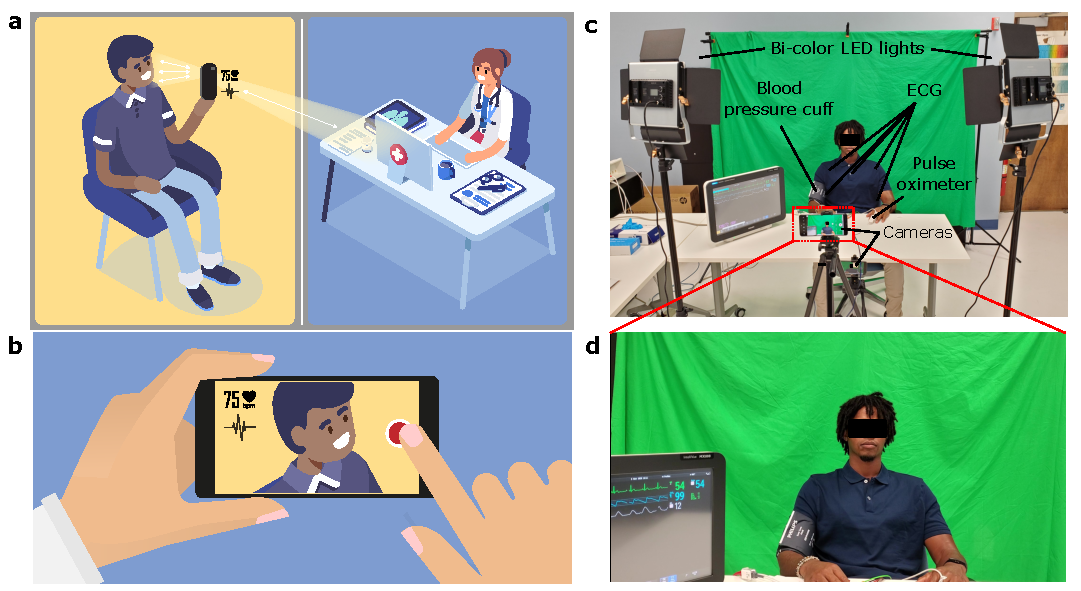
\includegraphics[width=\linewidth]{include/exp_setup.pdf}
    \caption{\textbf{Constructing a diverse remote vital sign monitoring dataset with a focus on telemedicine applications.} (a) Cartoon schematic depicting the telemedicine application for the proposed camera-based heart rate estimation. (b) Telemedicine video-conferencing applications can be integrated with a software toolkit to display patient BVP and HR. (c) Experimental setup employed during the construction of the VITAL dataset. Two bi-color LEDs are used for controlled illumination of the subject, and laboratory tube LEDs are used for ambient illumination. The Philips IntelliVue MX800 patient monitor is utilized for ground truth vital sign monitoring. Two smartphone cameras at differing viewing angles capture video of the subject. (d) Example frame from video captured by the smartphone camera. The subject wears a blood pressure cuff, 5-ECG leads, and a finger pulse oximeter, which is connected to the MX800 unit. Written consent was obtained from the subject for using their image in the publication.}
    \label{fig:exp_setup}
\end{figure}

To validate the performance of camera-based vital sign detectors, we construct the Vital-sign Imaging for Telemedicine AppLications (VITAL) dataset. The focus of this dataset is to represent diversity in factors that are relevant to telemedicine setups, including: (i) smartphone deployment, (ii) camera view angle, (iii) recording condition (lighting variation and talking), and (iv) patient demographic diversity. We address each of these aspects individually:

\begin{enumerate}[label=(\roman*)]
    \item \textbf{Smartphone deployment:} The ubiquity of smartphones globally has led to the development of patient portals, many of which can be accessed via smartphone applications that can be downloaded by patients (45–47). Such applications have been used for hosting telemedicine appointments. A deployable remote HR estimation solution with a focus on telemedicine must be able to work efficiently on smartphone cameras by considering factors including video compression (23, 42, 48) and algorithmic complexity. Moreover, the solution must achieve success independent of camera type. Hence, the VITAL dataset uses different smartphone cameras for each view angle. The use of more than one smartphone imager inspires the development of algorithms that can scale to a variety of device-agnostic telemedicine conditions. 
    \item \textbf{Camera view angle:} In a telemedicine setting, there can also be a variety of camera angles that the algorithm must work on. In order to facilitate this verification, the VITAL dataset consists of two camera view angles for all the videos of each subject (as seen in Figure~\ref{fig:exp_setup}).
    \item \textbf{Recording condition:} Another essential factor involves testing algorithms across a range of recording conditions, to promote the development of algorithms that can operate in the “wild”. The dataset consists of four recording conditions: (1) controlled lighting at 5600K (“cool” lighting) with the subject remaining stationary, (2) controlled lighting at 3200K (“warm” lighting) with the subject remaining stationary, (3) ambient room lighting- distributed white lighting- with the subject remaining stationary, and (4) ambient room lighting with the subject speaking. Additionally, a green screen backdrop is kept to potentially enable digital modification of background scenery.
    \item \textbf{Patient demographic diversity:} The VITAL dataset consists of 54 subjects spread across skin tone, age, gender, race, and ethnic backgrounds. Subject characteristics (gender, age, height, weight, body mass index, race, and ethnicity) are summarized in Table 1 using mean (SD), median (IQR), or frequency (\%), unless otherwise noted. For the purpose of this study, we split the subjects into three skin tone categories based on the Fitzpatrick (FP) skin type scale (49): light, consisting of skin tones in the FP 1 and 2 scales, medium, consisting of skin tones in the FP 3 and 4 scales, and dark, consisting of skin tones in the FP 5 and 6 scales. This aggregation allows for more relevant trends, since any two consecutive FP scale categories are reasonably close.
\end{enumerate}

The human study protocol was approved by the UCLA Institutional Review Board (IRB\#20-001025-AM-00001), and participants provided written informed consent to take part in the study. Figure~\ref{fig:exp_setup} shows the data collection setup. Each subject is made to sit on a height-adjustable chair, in the field of view of two cell-phone cameras (with different view angles): one camera (Samsung Galaxy S10) is perfectly front-on, while the other (Samsung Galaxy A51) is directly in front of the face, at a dip (lower) of 15 degrees. The front-on camera is placed approximately 130 cm from the subject, and the lower camera at a dip is approximately 90 cm from the subject. The height of the chair is chosen so that the subject is centered in the front-on frame. The controlled lights are set up on either side of the front-on camera, with a baseline of 100 centimeters between them.

As aforementioned, we record subjects using these cameras under four different scene conditions: (1) controlled lighting at 5600K (“cool” lighting) with the subject remaining stationary, (2) controlled lighting at 3200K (“warm” lighting) with the subject remaining stationary, (3) ambient room lighting (distributed white LED lighting) with the subject remaining stationary, and (4) ambient room lighting with the subject speaking. Controlled lighting is enabled by a pair of professional bi-color LED photography lights (Neewer Bi-Color 480 LED). The controlled lighting recording conditions were enabled with the room lights off, allowing for fine-tuned control over the illumination spectral properties. As incorporating controlled lighting only enables a front-facing illumination angle, two recording conditions in ambient room lighting were captured where the subject was lit more completely from several angles. The final recording condition involved variations in the subject, including talking, natural head movements, and facial expressions. Each scene recording session lasts for 2 minutes, for a total of 16 minutes of video footage across 8 videos. 

During data collection, volunteers are fitted with standard anesthesiology cardiopulmonary monitors: pulse oximeter (Red DCI, Masimo), blood pressure cuff (Comfort Care, Philips), and 5-lead electrocardiogram (Philips IntelliVue). To collect vital sign data, we utilize the Philips IntelliVue MX800 patient monitor to perform real time monitoring of four vital signs- HR, respiratory rate, oxygen saturation, and non-invasive continuous blood pressure- of which three waveforms are collected (ECG, PPG and respiration). We use the open source tool VSCapture (61) to collect data onto a computer using the MX800’s local area network communication protocol. The MX800’s estimated numeric values for the vital signs are sampled every 1 second, while the waveforms are sampled at variable frequencies. The ECG signal is sampled between 400-600 Hz, the PPG signal between 100-150Hz and the respiration between 40-60Hz.  Continuous non-invasive blood pressure estimates occur when the blood pressure cuff is activated, which is approximately once every 30 seconds. 

\section{Algorithmic principles of R-PPG}

\section{Denoising strategies}

\section{Diverse R-PPG}

